\chapter{Especificação de Requisitos de Sistema}
O funcionamento essencial do sistema, o que define seus requisitos funcionais, requer que a posição dos macacos seja possível de ser medida, armazenada e mostrada para o usuário.

Além desses, são levantados os requisitos não funcionais, que trabalham aspectos necessários e complementares para o bom funcionamento do sistema, muitas vezes previstos pelo público solicitante do mesmo.

No SIMIOS, os principais requisitos não funcionais foram apontados por pesquisadores biólogos e veterinários com experiência em monitoramento de macacos. Dentre eles, está que o peso da mochila que será anexada ao animal não deveria ultrapassar 10g para não influenciar em seu comportamento nem sobrecarregá-lo, visto que o principal grupo de foco (saguis) tem peso médio de 400g. Para isso, é interessante que todos os componentes da mochila sejam o mais leves possível.

Outra situação apontada é o fato de que toda vez que a bateria do aparelho tiver de ser trocada, o veterinário deverá capturar o macaco e sedá-lo, o que é bastante prejudicial para a confiança que o animal constrói pelo ser humano. Dessa forma, é desejável que a eficiência energética do dispositivo embarcado seja alta para que a bateria tenha de ser trocada com a menor frequência possível.

Além da mochila do animal, espera-se que os dados coletados sejam confiáveis. Isso envolve garantir a autenticidade e a ausência de erros, ou seja, que eles estejam sendo de fato enviados íntegros pelo macaco a quem estão associados. Assim, evita-se casos em que o dispositivo possa ter sido removido acidentalmente e, por exemplo, enroscado em uma árvore ou em que existam interferências ruidosas no sinal capazes de alterar significativamente as medições enviadas. Também é relevante que o acesso à informação seja possível somente para pessoas autorizadas, envolvendo conceitos como autenticação e codificação.

SIMIOS é um sistema que, estruturalmente, poderia ser contextualizado em praticamente qualquer aplicação que se tenha algo a ser rastreado, seja um ser vivo ou não, para qual a precisão do GPS seja insuficiente. Portanto, de maneira geral, também é interessante que o sistema tenha escalabilidade em todos os aspectos - que os dispositivos embarcados nos animais possuam sensores diversos e que, possivelmente, toda a aplicação suporte que uma quantidade maior de variáveis e de usuários seja inserida.

Por fim, é sempre relevante que a interface com o usuário siga princípios de UX, especialmente se considerando que uma quantidade grande de dados deve ser visualizada de forma intuitiva e simples pelo pesquisador.

\begin{figure}[ht]
  \centering
    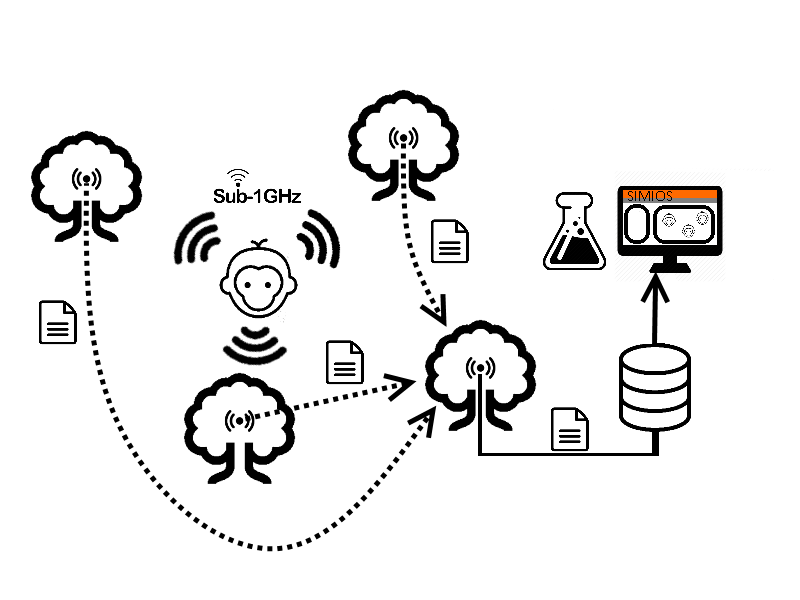
\includegraphics[scale=1]{esquematico}
  \caption{Resumo gráfico do sistema (Fonte: autores)}
\end{figure}
\FloatBarrier